\documentclass{article}

\usepackage{authblk}
\usepackage{graphicx}

\title{
    Comunicação por Computador \\
    \large{Trabalho Prático 1}
}
\author{
    Marco Costa A93283
}
\date{27 de outubro de 2021}
\affil{
    Universidade do Minho
}

\begin{document}
        \maketitle
    \section*{Respostas}
        \subsection*{1}
            {
                \centering
                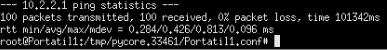
\includegraphics[width=12cm]{images/ping-portatil.png}
                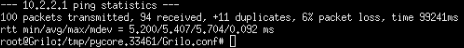
\includegraphics[width=12cm]{images/ping-grilo.png}
                \par
            }
                Como podemos ver nas imagens o nó \textit{Grilo}, que no \textit{CORE} lhe foi dada
            uma conexão com 10\% de duplicação e 5\% de packet loss, de 100 pacotes enviados apenas recebeu
            94 mais 11 pacotes duplicados. Isto contrasta com o \textit{Portatil1} que com uma conexão boa conseguiu
            receber os 100 pacotes de resposta sem qualquer duplicação ou perda destes.\par

                Mais interessante é o resultado destes problemas de conexão no \textit{rtt(round-trip time)} em que se pode verificar
            que o \textit{Grilo} teve valores significativamente mais elevados que a sua contraparte. Apesar disto o \textit{Grilo} demorou
            menos 2101ms a executar.
        \subsection*{2}
            {
                \centering
                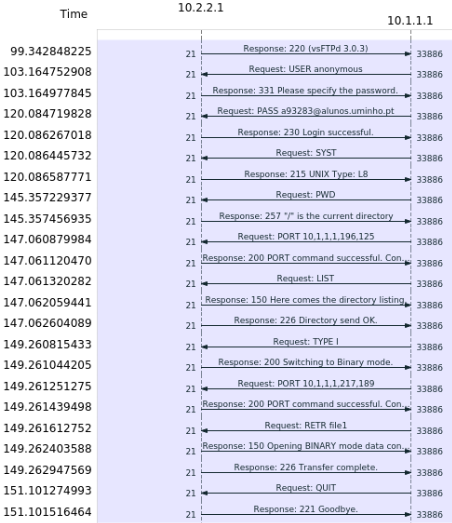
\includegraphics[width=12cm]{images/ftp-flow-graph.png}
                \par
            }
                Através do diagrama produzido pelo wireshark podemos ver toda a comunicação ftp feita entre o \textit{Portatil1} e o \textit{Servidor1}.

            Aqui é possível identificar o processo de login todos os comandos executados, incluíndo a transferência do ficheiro feita através de um pedido \textbf{\textit{RETR}}, e também o término de conexão
            feito com um pedido \textbf{\textit{QUIT}}.
                
                Para além disso o diagrama mostra que a conexão do lado do servidor está a ser feita na porta 21 que é reservada para o protocolo ftp.
        \subsection*{3}
            {
                \centering
                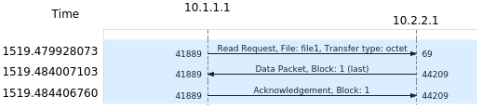
\includegraphics[width=12cm]{images/tftp-wireshark-flow-graph.png}
                \par
            }
                O protocolo tftp mostra-se bem mais simples que o ftp tendo sido apenas trocados 3 pacotes.
            A conexão é iniciada com um \textit{Read Request}, o servidor envia o ficheiro e, por fim, o portátil responde com um \textit{Acknoulegment}.

            Tal como no exercício anterior podemos conferir no diagrama que o servidor inicia a conexão na porta 69 que corresponde a porta reservada para o tftp. No entanto a conexão muda para a porta 44209.
        \subsection*{4}
                Após o uso dos quatro programas podemos concluir que o mais seguro é o sftp pelo seu uso do protocolo ssh que encripta toda a comunicação entre despositivos.

                Em termos de simplicidade http é o melhor devido ao facto de que só é necessário enviar um pacote \textit{GET} e o servidor retorna o ficheiro.

                No que toca à camada de transporte e eficiência o atftp destaca-se por ser o único que usa udp.
\end{document}
